\documentclass[12pt,twocolumn]{article}
	\usepackage[portuguese]{babel}
	\usepackage[utf8]{inputenc}
	\usepackage[T1]{fontenc}
	
	\usepackage[legalpaper, left=1cm, right=1cm, top=2cm, bottom=2cm]{geometry}	
	\usepackage{multicol}
	
	\usepackage{lipsum}
	
	\usepackage{wrapfig} 
	\usepackage{graphicx}
	\graphicspath{{./fig/}}
	
	\newcommand{\msg}[1]{\textsf{\textit{#1}}}

%opening
\title{Multicast Confiável}
\author{Guilherme Akira Demenech Mori}

\begin{document}	
	
	%\sffamily 
	
	%\begin{multicols}{2}		
		
		\maketitle	
	
		\begin{abstract}
			
		\end{abstract}
	
		\tableofcontents
		
		\listoffigures
	
	%\end{multicols}

	%\begin{multicols}{3}
	
		\section*{Contextualização}
			Comunicação é um aspecto essencial da vida humana na Terra.
			Seres humanos, assim como vários outros animais sociais, dependem das relações com outros indivíduos.
			Vemos essa dependência, material e psicológica, se expressar nos mais diversos contextos: divisão do trabalho, amizade, afetividade etc.  
			
			O desenvolvimento da linguagem demonstra a importância da comunicação para a sociedade.
			De fato, é difícil imaginar a organização social sem alguma padronização de comunicação.
			Os protocolos de telecomunicação criam padrões muito mais restritivos que a linguagem natural (isto é, os idiomas humanos) e permitem transmissão de dados por longas distâncias entre dispositivos de inúmeros fabricantes.						  
	
			\subsection{Definição do problema}
				Utilizando somente comunicação ponto-a-ponto, propor protocolos que garantam a entrega a múltiplos hosts ou que detectem quais apresentaram falhas.  		
				Deve-se buscar reduzir o tráfego da rede como um todo e também a sobrecarga de hosts individuais.
				
				O host remetente deve identificar quais destinatários confirmaram recebimento e qual foi o intervalo de tempo para detectar falha. 
				Da mesma forma, os hosts destinatários devem exibir a mensagem recebida somente uma vez, confirmando recebimento.
				
				Os hosts poderão ser identificados por nomes, para facilitar a diferenciação entre eles e para auxiliar o(a) usuário(a) humano(a) a memorizá-los.							
						
		\section{Unicast}
		
			Para se enviar uma mensagem para somente um destinatário, basta que o host envie e aguarde confirmação.  
			A Figura~\ref{fig:unicast} representa o unicast bem sucedido entre dois hosts.
			Um host envia a mensagem e o outro confirma o recebimento com \msg{ok}.
			
			\begin{figure}[htp]%{R}{0.6\linewidth}%			
				\centering
				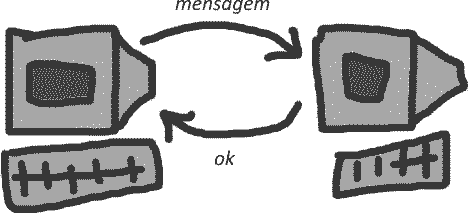
\includegraphics[width=0.9\linewidth]{unicast.png}%
				\caption{Unicast}%
				\label{fig:unicast}				
			\end{figure}	
		
			Caso seja necessário garantir o unicast, basta que o host remetente reenvie a mensagem até que ele receba a confirmação.
			Assim que ele receber a confirmação, simplesmente para de enviar a mensagem.
			O destinatário, ao identificar que recebeu a mensagem repetida, entende que o remetente não recebeu a confirmação e a reenvia somente uma vez.
			Quando o destinatário parar de receber reenvios da mensagem, ele compreende que o remetente finalmente recebeu a confirmação.
			
			É importante ressaltar que o destinatário não reenvia \msg{ok} por si só. 
			Ele só repete a confirmação quando recebe novamente a mensagem, assim, não é preciso que o destinatário confirme que recebeu a confirmação.
		
		\section{Multicast}
		
		\section{Propostas de protocolo}	
		
			
				
			
	%\end{multicols}
\end{document}
